\chapter{Message Passing using Channels} 


We saw in the last chapter that we need some way to provide for
\emph{disciplined} interaction between threads, to avoid threads interfering
with one another.  In this book, we will see three basic ways to achieve this:
message passing, monitors and semaphores.  At a higher level of abstraction,
we will also see how to use concurrent datatypes.

We will start with message passing.  In my opinion, it is the most intuitive
approach: one thread can send a message to another thread.  
In addition, message passing is  necessary for distributed computing, and also
works well with loosely coupled systems.  

A downside is that message passing tends to be slower than other approaches,
because there is an overhead in the sending and receiving of messages.
However, it is a good paradigm to start with, to get used to thinking about
concurrent programs.

The basic idea is that programs are composed of components, which might be
either threads (i.e.~sharing an address space) or processes (with distinct
address spaces, possibly on different computers).  These processes communicate
only by sending and receiving messages over \emph{channels}.  In this book, we
will be dealing with threads; but the same techniques can be used with
processes. 

%%%%%

Think of a channel as a directional wire.  Messages are sent at one end, and
received at the other end. 

%% \item At one end there is an output port, at the other an input port.
%% %
%% \begin{center}
%% \begin{tikzpicture}
%% \draw (0,0) node[draw] (sender) {\scalashape chan!v};
%% \draw (4.5,0) node[draw] (receiver) {\scalashape chan?()};
%% \draw[->] (sender) -- 
%%   node[above,near start]{\small outport} 
%%   node[above,near end]{\small inport} (receiver);
%% \end{tikzpicture}
%% \end{center}

%% \item Values sent at the outport end (using |chan!v|) are received at the
%%   inport end (using |chan?()|), in the same order.

%% \item
%% Channels can be either synchronous or asynchronous; we will use a mix in this
%% course.
%% \end{itemize}
%% \end{slide}

%%%%%

In SCL, \SCALA{Chan[A]} is the type of channels that pass data of
type~\SCALA{A}.  This has two concrete subtypes: |SyncChan[A]|, of synchronous
channels; and |BuffChan[A]|, of buffered (or asynchronous) channels.  We will
start by describing synchronous channels, and later describe buffered
channels. 

The command
\begin{scala}
  val chan = new SyncChan[A]
\end{scala}
defines |chan| to be a synchronous channel passing data of type~|A|.  Then the
command 
\begin{scala}
  chan!v
\end{scala}
sends the value \SCALA{v} on \SCALA{chan}.  The expression
\begin{scala}
  chan?()
\end{scala}
receives a value from~\SCALA{chan} and returns it.  The communication is
\emph{synchronous}: whichever part is executed first waits for the other; both
then proceed.  Thus the send and receive appear to take place at the same
time.  

%%%%%

For example, the following program prints the number 42 (in a round-about
way): 
\begin{scala}
  val chan = new SyncChan[Int]
  run(thread{ chan!42 } || thread{ println(chan?()) }) 
\end{scala}
%
This runs two threads: the first thread sends 42 on the channel; the second
thread receives a value on the channel, and prints it.

%%%%%

As another example, here's a thread that inputs values from the channel
\SCALA{in}, and outputs them on the channel~\SCALA{out}:
%
\begin{scala}
def copy[A](in: SyncChan[A], out: SyncChan[A]) = thread{
  while(true){ val x = in?(); out!x }
}
\end{scala}
%
(The function that creates the thread is parameterised by the channels, and by
the type~|A| of those channels.)
%
We could have written the body of \SCALA{copy} as simply:
\begin{scala}
  while(true) out!(in?()) 
\end{scala}
Note that in both forms, the communication on |in| can proceed even if no
thread is yet ready to receive on |out|.

%%%%%

A channel is simply an \SCALA{InPort} (something from which threads can
receive) and an \SCALA{OutPort} (something on which threads can send).  A
channel is composed of an |InPort| and an |OutPort|.
Note that the terminology ``|InPort|'' and ``|OutPort|'' refer to the point of
view of \emph{threads}, not channels: a thread receives values in on an
|InPort|, and sends values out on an |OutPort|; however, a value is put into a
channel on an |OutPort|, and passed out on an |InPort|.

Figure~\ref{fig:channel-types} outlines the relevant types.  (The definition
of |Chan[A]| uses multiple inheritance: it inherits definitions from both
|InPort[A]| and |OutPort[A]|.)  The types \SCALA{InPort[A]} and
\SCALA{OutPort[A]} can be abbreviated as \SCALA{??[A]} and~\SCALA{!![A]}.

%%%%%%

\begin{figure}
\begin{scala}
package ox.scl.channel

trait InPort[A]{ def ?(): A; ... }
        
trait OutPort[A]{ def !(value: A): Unit; ... }
  
trait Chan[A] extends InPort[A] with OutPort[A]{ ... }

class SyncChan[A] extends Chan[A]{...} 
\end{scala}
\caption{Outline of the types of channels.}
\label{fig:channel-types}
\end{figure}

%%%%%

The earlier function \SCALA{copy} uses only the \SCALA{InPort} of \SCALA{in}
and the \SCALA{OutPort} of \SCALA{out}.  We therefore could have written the
definition as:
%
\begin{scala}
def copy[A](in: ??[A], out: !![A]) = thread{ 
  while(true) out!(in?()) 
}
\end{scala}
%
This signature makes clear what the thread does with each channel, and so
helps with documentation (the names of the channels also help).  In addition,
this style provides some  type safety: if, for example, the code tries to send
on~|in|, the compiler will give a type error. 

%%%%%

Figure~\ref{fig:Mults4} gives a slightly larger example.  The function
|console(in)| defines a thread that repeatedly reads a value from \SCALA{in}
and writes it to standard output.  The function \SCALA{nats(out)} defines a
thread that sends the natural numbers, in order, on \SCALA{out}.  The function
\SCALA{alts(in, out)} defines a thread that copies alternate values read from
\SCALA{in} to \SCALA{out}.

%%%%%

\begin{figure}
\begin{scala}
import ox.scl._

object Mults4{
  def console[A](in: ??[A]) = thread{ while(true) println(in?()) }

  def nats(out: !![Int]) = thread{ 
    var n = 0; while(true){ out!n; n += 1 }
  }

  def alts[A](in: ??[A], out: !![A]) = thread{ 
    while(true){ out!(in?()); in?() } 
  }

  private val x1, x2, x4 = new SyncChan[Int]

  def system = nats(x1) || alts(x1, x2) || alts(x2, x4) || console(x4)

  def main(args: Array[String]) = run(system)
}
\end{scala}
\caption{Printing multiples of four.}
\label{fig:Mults4}
\end{figure}

%%%%%

The definition of |system| puts the components together as illustrated below.  
%
\begin{center}
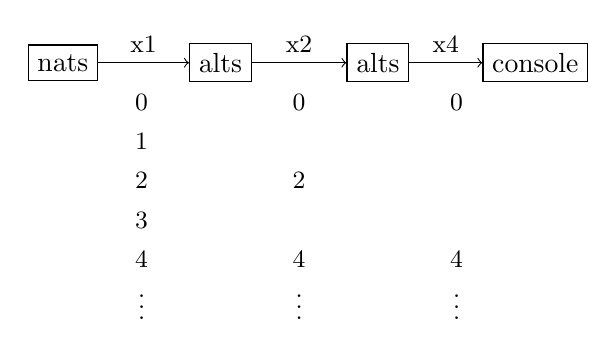
\begin{tikzpicture}
\draw (0,0) node[draw] (nats) {\scalashape nats};
\draw (nats)++(2,0) node[draw] (alts1) {\scalashape alts};
\draw[->] (nats) -- node[above]{\small\scalashape x1} (alts1);
\draw (alts1)++(2,0) node[draw] (alts2) {\scalashape alts};
\draw[->] (alts1) -- node[above]{\small\scalashape x2} (alts2);
\draw (alts2)++(2,0) node[draw] (console) {\scalashape console};
\draw[->] (alts2) -- node[above]{\small\scalashape x4} (console);
%
\draw (nats)++(1,-0.5) node {\small\scalashape 0};
\draw (nats)++(1,-1) node {\small\scalashape 1};
\draw (nats)++(1,-1.5) node {\small\scalashape 2};
\draw (nats)++(1,-2) node {\small\scalashape 3};
\draw (nats)++(1,-2.5) node {\small\scalashape 4};
\draw (nats)++(1,-3) node {\small\scalashape \vdots};
%
\draw (alts1)++(1,-0.5) node {\small\scalashape 0};
\draw (alts1)++(1,-1.5) node {\small\scalashape 2};
\draw (alts1)++(1,-2.5) node {\small\scalashape 4};
\draw (alts1)++(1,-3) node {\small\scalashape \vdots};
%
\draw (alts2)++(1,-0.5) node {\small\scalashape 0};
\draw (alts2)++(1,-2.5) node {\small\scalashape 4};
\draw (alts2)++(1,-3) node {\small\scalashape \vdots};
\end{tikzpicture}
\end{center}
%
The |nats| thread outputs the natural numbers on~|x1|.  The first instance of
|alts| receives these, and outputs every other value, i.e.~the even natural
numbers, on~|x2|.  The second instance of |alts| receives these, and outputs
every other value, i.e.~the multiples of~4, on~|x4|.  |console| receives these
and prints them.  Thus the overall effect is to print the (non-negative)
multiples of~4.

%%%%%%%%%%%%%%%%%%%%%%%%%%%%%%%%%%%%%%%%%%%%%%%%%%%%%%%%%%%%

\section{Buffered channels}

In the previous example, we used synchronous channels.  In effect, on each
channel, the send and receive of each value happen at the same time: the
sender and receiver \emph{synchronise} on the communication.
%
Using synchronous channels can make programs easier to understand: it helps us
to relate the states in different components.

By contrast, buffered channels normally allow a send to happen, even if there
is no thread ready to receive: the sender can return immediately, and the
channel stores the values until a receiver is ready to receive them.  In
particular, the channel ensures the messages are received in the same order in
which they are sent: the channel acts as a first-in first-out buffer.

However, the implementation of buffered channels imposes a bound on the number
of messages that can be buffered.  Suppose we did not have such a bound, and
imagine a scenario where the sender sent messages much faster than the
receiver could deal with them.  Then the buffered channel will hold more and
more messages, consuming more and more memory, possibly until all available
memory is used.  With a bounded buffered channel, once the bound is reached,
the sender is blocked until the receiver is ready to receive one of the
earlier messages. 

%%%%%

\heading{Buffered channels}

The class of buffered channels is defined as follows.
%
\begin{scala}
class BuffChan[A: scala.reflect.ClassTag](size: Int) extends Chan[A]
\end{scala}
%
Thus a declaration such as
\begin{scala}
val chan = new BuffChan[Int](size)
\end{scala}
defines a new buffered channel, passing |Int|s, able to hold at most |size|
messages.

In the multiples-of-four example, we could have defined the channels as 
%
\begin{scala}
  val x1, x2, x4 = new BuffChan[Int](10)
\end{scala}
%
Making the channels buffered might help to overcome inconsistencies in the
speeds of threads.  For example, is one thread is suspended, its neighbours
will be able to continue for a while.

The ``|[A: scala.reflect.ClassTag]|'' in the declaration of |BuffChan| needs
some explanation. Internally, a {\scalashape BuffChan} stores the buffered
messages in an array.  This means that the runtime implementation needs to
construct an |Array[A]|.  However, in order to do this, it needs to have what
is known as a |ClassTag| for~|A|, essentially information that tells the
runtime what |A| is.  If {\scalashape A} is a concrete type, e.g.~{\scalashape
  Int}, then the runtime implementation can construct the {\scalashape
  ClassTag} itself.  In such --- very common --- cases, you don't need to
provide the |ClassTag|: you can happily ignore the issue.  However, if
{\scalashape A} is declared as a polymorphic type in some enclosing
definition, it should be given the type bound {\scalashape A:
  scala.reflect.ClassTag}, and the compiler will ensure a {\scalashape
  ClassTag} is available.  For example, here's a version of the earlier |copy|
function that uses buffered channels: the type parameter |A| of |copy| needs
to be given the type bound.
%
\begin{scala}
def copy[A: scala.Reflect.ClassTag](in: BuffChan[A], out: BuffChan[A]) = thread{
  while(true){ val x = in?(); out!x }
}
\end{scala}
%
When |copy| is called with a concrete type for~|A|, the runtime will provide
the |ClassTag|. 



% %%%%%%%%%%%%%%%%%%%%%%%%%%%%%%%%%%%%%%%%%%%%%%%%%%%%%%%%%%%%

\heading{tee}

The following thread inputs values on~\SCALA{in}, and outputs on
both~\SCALA{out1} and \SCALA{out2}.
%
\begin{scala}
def tee[A](in: ??[A], out1: !![A], out2: !![A]) = thread{
  while(true){ val v = in?(); out1!v; out2!v }
}
\end{scala}

The above version of \SCALA{tee} outputs on its \SCALA{out1} channel before
its \SCALA{out2} channel.  What happens if we use this in the context of some
larger system that inputs on \SCALA{out2} before \SCALA{out1}?  For example:
\begin{scala}
val in, out1, out2 = new SyncChan[Int]
run( tee(in, out1, out2) || thread{ println(out2?() + out1?()) } )
\end{scala}

% %%%%%

Generic components should place as few assumptions as possible upon the
network in which they are placed.  The following version of |tee| performs the
outputs concurrently, i.e.~in either order.
%
\begin{scala}
def tee[A](in: ??[A], out1: !![A], out2: !![A]) = thread{
  while(true){ 
    val v = in?()
    run(thread{out1!v} || thread{out2!v}) 
  }
}
\end{scala}

However, creating and running two new threads is moderately expensive.  In
specific settings, it might be more efficient and easier to perform the
outputs in a fixed order.

%%%%%%%%%%%%%%%%%%%%%%%%%%%%%%%%%%%%%%%%%%%%%%%%%%%%%%%% %%%%%

\section{Closing channels}

Often a component has to process a finite stream of data.  But how should the
end of the stream be signalled?  One way might be to send a special
``end-of-stream'' value.  But that assumes that we can find such a value, that
won't be sent as a valid piece of data; and it will require additional
programming to send that value, and for the receiver to recognise it and act
appropriately. 

An alternative way to indicate the end of the data stream is for the sender to
close the channel.  But also, a receiver can close a channel, to signal to the
sender that it is unable to accept more data.

In SCL, if |in| is an |InPort| (e.g.~a channel), then |in.close| closes it.
%
If |out| is an |OutPort| (e.g.~a channel), then |out.endOfStream| closes it
for sending.  For a synchronous channel, this also closes it for receiving.
However, for a buffered channel, other threads can continue to receive until
the buffer becomes empty, at which point the channel becomes fully closed.

%%%%%

If a thread tries to send or receive on a channel that has been closed, it
throws a |Closed| exception, a subclass of the |Stopped| exception class.
(Well see another subclass of |Stopped| in Chapter~\ref{chap:alts}.)

Threads should normally catch such exceptions, and then do the right thing.
For a receiver, if the closing represents the end of the data stream, then
typically the thread should just close.  If the thread is part of a larger
network, such as a pipeline, then typically the thread should close channels
to other components, to signal to the next component in line that the stream
is closed.

%% If such closing is possible, the thread should handle it appropriately,
%% normally closing its channels to pass the message on. 

Here's a new version of |alts| that does this.
%
\begin{scala}
def alts[A](in: ??[A], out: !![A]) = thread{ 
  try{ while(true){ out!(in?()); in?() } } 
  catch{ case _: Closed => in.close; out.endOfStream }
}
\end{scala}
% 
If either sending or receiving fails, because the channel has been closed, the
thread exits the loop, and closes both channels.  Note that closing a channel
that is already closed has no effect.

Note also that there's no need to close a channel that is about to go out of
scope and be garbage collected. 

The above pattern is sufficiently common, that there's a construct to capture
it.
%
\begin{scala}
  repeat{ <command> }
\end{scala}
%
behaves much like
\begin{scala}
  while(true){ <command> }
\end{scala}
but terminates cleanly if \SCALA{<command>} throws a \SCALA{Stopped}
exception.

For example:
%
\begin{scala}
def alts[A](in: ??[A], out: !![A]) = thread{ 
  repeat{ out!(in?()); in?() } 
  in.close; out.endOfStream
}
\end{scala}

%%%%%

The construct
%
\begin{scala}
  repeat(guard){ <command> }
\end{scala}
%
behaves much like
\begin{scala}
  while(guard){ <command> }
\end{scala}
but terminates cleanly if \SCALA{<command>} throws a \SCALA{Stopped}
exception.

A closed channel~|c| can be reopened using the construct
\begin{scala}
  c.reopen
\end{scala}
%
This has a precondition that the channel is indeed closed, and that no thread
is trying to send or receive on it.  This allows channels to be reused.

It is possible to test whether a channel~|c| is closed using
%
\begin{scala}
  c.isClosed
\end{scala}
 % Channels; buffered channels
\section{Closing channels}

Often a component has to process a finite stream of data.  But how should the
end of the stream be signalled?  One way might be to send a special
``end-of-stream'' value.  But that assumes that we can find such a value, that
won't be sent as a valid piece of data; and it will require additional
programming to send that value, and for the receiver to recognise it and act
appropriately. 

Further, it can sometimes be useful for a receiver to indicate to the sender
that it is unable to accept any more data.

The way we deal with each of these scenarios is for the relevant thread to
close the channel. 
%
In SCL, if |in| is an |InPort| (e.g.~a channel), then |in.close()| closes it.
%
If |out| is an |OutPort| (e.g.~a channel), then |out.endOfStream()| closes it
for sending.  For a synchronous channel, this also closes it for receiving.
However, for a buffered channel, other threads can continue to receive until
the buffer becomes empty, at which point the channel becomes fully closed.

%%%%%

If a thread tries to send or receive on a channel that has been closed, it
throws a |Closed| exception, a subclass of the |Stopped| exception class.
(We will see another subclass of |Stopped| in Chapter~\ref{chap:alts}.)

Threads should normally catch such exceptions, and then do the right thing.
For a receiver, if the closing represents the end of the data stream, then
typically the thread should terminate.  But if the thread is part of a larger
network, such as a pipeline, then typically the thread should first close
channels to other components, to signal to the next component in line that the
stream is closed.

%% If such closing is possible, the thread should handle it appropriately,
%% normally closing its channels to pass the message on. 

Here's a new version of |alts| that does this.
%
\begin{scala}
  def alts[A](in: ??[A], out: !![A]) = thread("alts"){ 
    try{ while(true){ out!(in?()); in?() } } 
    catch{ case _: Closed => in.close(); out.endOfStream() }
  }
\end{scala}
% 
If either sending or receiving fails, because the channel has been closed, the
thread exits the loop, and closes both channels.  Note that closing a channel
that is already closed has no effect.

Note also that there's no need to close a channel that is about to go out of
scope and be garbage collected. 

The above pattern is sufficiently common, that there's a construct to capture
it.
%
\begin{scala}
  repeat{ <command> }
\end{scala}
%
behaves much like
\begin{scala}
  while(true){ <command> }
\end{scala}
but terminates cleanly if \SCALA{<command>} throws a \SCALA{Stopped}
exception.
Figure~\ref{fig:BoundedMults4} illustrates this for the |alts| function.
%% For example:
%% %
%% \begin{scala}
%% def alts[A](in: ??[A], out: !![A]) = thread{ 
%%   repeat{ out!(in?()); in?() } 
%%   in.close(); out.endOfStream()
%% }
%% \end{scala}

%%%%%

It's sometimes useful to exit a loop for some reason other than a channel
being closed.  The construct
%
\begin{scala}
  repeat(guard){ <command> }
\end{scala}
%
behaves much like
\begin{scala}
  while(guard){ <command> }
\end{scala}
but terminates cleanly if \SCALA{<command>} throws a \SCALA{Stopped}
exception.

%%%%%%%%%%

Figure~\ref{fig:BoundedMults4} illustrates the technique of closing channels
via a version of the multiples-of-four example that prints up to some maximum
value~|max|, and then terminates cleanly.  This works by inserting a new
component into the pipeline, to close down the network once a value greater
than |max| is reached, as illustrated below.
%
\begin{center}
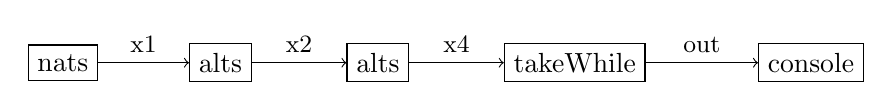
\begin{tikzpicture}
\draw (0,0) node[draw] (nats) {\scalashape nats};
\draw (nats)++(2,0) node[draw] (alts1) {\scalashape alts};
\draw[->] (nats) -- node[above]{\small\scalashape x1} (alts1);
\draw (alts1)++(2,0) node[draw] (alts2) {\scalashape alts};
\draw[->] (alts1) -- node[above]{\small\scalashape x2} (alts2);
\draw (alts2)++(2.5,0) node[draw] (takeWhile) {\scalashape takeWhile};
\draw[->] (alts2) -- node[above]{\small\scalashape x4} (takeWhile);
\draw (takeWhile)++(3,0) node[draw] (console) {\scalashape console};
\draw[->] (takeWhile) -- node[above]{\small\scalashape out} (console);
%
%% \draw (nats)++(1,-0.5) node {\small\scalashape 0};
%% \draw (nats)++(1,-1) node {\small\scalashape 1};
%% \draw (nats)++(1,-1.5) node {\small\scalashape 2};
%% \draw (nats)++(1,-2) node {\small\scalashape 3};
%% \draw (nats)++(1,-2.5) node {\small\scalashape 4};
%% \draw (nats)++(1,-3) node {\small\scalashape \vdots};
%% %
%% \draw (alts1)++(1,-0.5) node {\small\scalashape 0};
%% \draw (alts1)++(1,-1.5) node {\small\scalashape 2};
%% \draw (alts1)++(1,-2.5) node {\small\scalashape 4};
%% \draw (alts1)++(1,-3) node {\small\scalashape \vdots};
%% %
%% \draw (alts2)++(1,-0.5) node {\small\scalashape 0};
%% \draw (alts2)++(1,-2.5) node {\small\scalashape 4};
%% \draw (alts2)++(1,-3) node {\small\scalashape \vdots};
\end{tikzpicture}
\end{center}

%%%%%

\begin{figure}
\begin{scala}
object BoundedMults4{
  def nats(max: Int, out: !![Int]) = thread("nats"){ 
    var n = 0
    repeat{ out!n; n += 1 }
  }

  def alts[A](in: ??[A], out: !![A]) = thread("alts"){ 
    repeat{ out!(in?()); in?() }
    in.close(); out.endOfStream()
  }

  def console[A](in: ??[A]) = thread("console"){ repeat{ println(in?()) } }

  def takeWhile[A](p: A => Boolean, in: ??[A], out: !![A]) = thread("takeWhile"){
    var done = false
    repeat(!done){ val x = in?(); if(p(x)) out!x else done = true }
    in.close(); out.endOfStream()
  }

  def system(max: Int) = {
    val x1, x2, x4, out = new SyncChan[Int]
    nats(max, x1) || alts(x1, x2) || alts(x2, x4) || 
      takeWhile((x: Int) => x <= max, x4, out) || console(out)
  }

  def main(args: Array[String]) = {
    val max = args(0).toInt; run(system(max))
  }
}
\end{scala}
\caption{Printing multiples of four, up to some maximum value.}
\label{fig:BoundedMults4}
\end{figure}

%%%%%

In fact, the new component is an instance of a more general pattern.  The
function |takeWhile(p, in, out)| copies data from~|in| to~|out| while all
values satisfy the predicate~|p| (the type \protect\SCALA{A => B}
  represents functions from~{\scalashape A} to~{\scalashape B}); it then
closes the channels.  

The other components are adapted to handle the closing of channels, using
|repeat|.  The |alts| components also close their channels, to indicate to
their neighbours that the system is terminating (in fact, the
``|out.endOfStream()|'' is unnecessary in this case because that part of the
network is closing in an upstream direction). 

The function |system| creates the channels and puts the components together in
parallel.  (In the first parameter of |takeWhile|, the notation \SCALA{(x:
  Int) => x <= max} represents the function that takes an |Int| argument~|x|,
and returns the result of the test |x <= max|.)

\begin{instruction}
Make sure you understand how the termination signal is propagated through the
system. 
\end{instruction}
%\medskip

There are two other operations on channels related to closing. 
It is possible to test whether a channel~|c| is closed using the expression
%
\begin{scala}
  c.isClosed
\end{scala}
%
A closed channel~|c| can be reopened using the construct
\begin{scala}
  c.reopen()
\end{scala}
%
This has a precondition that the channel is indeed closed, and that no thread
is trying to send or receive on it.  This allows channels to be reused.

\framebox{Cut above?}

%%%%%%%%%%%%%%%%%%%%%%%%%%%%%%%%%%%%%%%%%%%%%%%%%%%%%%%

\section{Example: producing the natural numbers}

We now consider another example of fine-grained concurrency, a circuit that
outputs the natural numbers.  The circuit is depicted below, and the code is
in Figure~\ref{fig:NatsCircuit}. 

\begin{center}
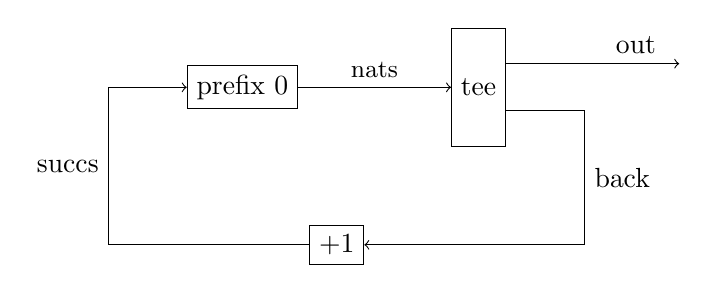
\begin{tikzpicture}
\draw(0,0) node[draw] (prefix) {\scalashape prefix 0};
% tee
\draw(prefix) ++(3,0) node[draw, minimum height = 15mm] (tee) {\scalashape tee};
\draw[->] (prefix) -- node[above]{\small\scalashape nats} (tee);
\draw[->] (tee.east)++(0,0.3) -- 
  node[above, near end]{\scalashape out} ++ (2.2,0);
% +1
\draw(prefix) ++ (1.2,-2) node[draw] (succ) {\scalashape +1};
\draw[->] (tee.east)++(0,-0.3) -- ++ (1.0,0) |-  
  node[right, near start]{\scalashape back} (succ);
\draw[->] (succ) -- ++(-2.9,0) |- 
  node[left, near start]{\scalashape succs} (prefix);
\end{tikzpicture}
\end{center}

%%%%%

\begin{figure}
\begin{scala}
object NatsCircuit{
  def console[A](in: ??[A]) = thread("console"){ repeat{ println(in?()) } }

  def prefix[A](x: A, in: ??[A], out: !![A]) = thread("prefix"){
    out!x; repeat{ out!in?() }
  }

  def tee[A](in: ??[A], out1: !![A], out2: !![A]) = thread("tee"){
    repeat{ val x = in?(); out1!x; out2!x }
  }

  def map[A,B](f: A => B, in: ??[A], out: !![B]) = thread("map"){
    repeat{ out!(f(in?())) }
  }

  def nats(out: !![Int]): ThreadGroup = {
    val nats, succs, back = new SyncChan[Int]
    prefix(0, succs, nats) || tee(nats, out, back) ||
      map(((x: Int) => x+1), back, succs)
  }

  def system: ThreadGroup = {
    val c = new SyncChan[Int]; nats(c) || console(c)
  }

  def main(args: Array[String]) = run(system)
}
\end{scala}
\caption{A concurrent circuit that outputs the natural numbers.}
\label{fig:NatsCircuit}
\end{figure}

The component labelled ``|prefix 0|'' copies values from |succs| to |nats|,
prefixing them with the value~|0|; it is produced using the function |prefix|.
The component labelled ``|tee|'' copies values from |nats| to both |out| and
|back|; it is produced using the function |tee|.  The component labelled
``|+1|'' adds~|1| to each value it receives on |back|, and outputs the result
on |succs|; it is produced by the function |map|, which generalises the
particular functionality we need, by applying the function~|f| to each value
it receives.  Then |nats| puts the components together, and |system| connects
|nats| to a console component.

Note that the circuit is cyclic.  Initially, |prefix 0| will produce~|0|; this
will be output and passed to |+1|.  The |+1| component will pass~|1| back to
|prefix 0|, via which it will be output and passed round the circuit.  And so
on.  In particular, it is important that |prefix 0| can send \emph{before} it
receives any value.  If every component started by trying to receive a value,
none would succeed, and the circuit would be deadlocked. 

\begin{instruction}
Make sure you understand how the circuit works, and how values propagate
round.
\end{instruction}

The above version of \SCALA{tee} outputs on its \SCALA{out1} channel before
its \SCALA{out2} channel.  That definition is fine in the context of the
circuit in question.  However, it could go wrong if used in the context of
some larger system that inputs on \SCALA{out2} before \SCALA{out1}.  For
example consider the following:
%
\begin{scala}
  val in, out1, out2 = new SyncChan[Int]
  def printer = thread("printer"){ println(out2?() + out1?()) } 
  run( tee(in, out1, out2) || printer)
\end{scala}
%
The printer thread will try to input on |out2| first (because |+| evaluates
its left-hand argument first).  But that means the system will get into a
deadlocked state, where the |tee| is blocked, trying to send on |out1|, and
the printer is blocked trying to receive on |out2|.  (Recall that in such
situations, typing \texttt{Ctrl}+$\backslash$ in the terminal produces a
thread dump, giving information about the running threads, which can be useful
for debugging.)

%% % %%%%%

%% Generic components should place as few assumptions as possible upon the
%% network in which they are placed. 
The following version of |tee| performs the outputs concurrently, which means
they can happen in either order.
%
\begin{mysamepage}
\begin{scala}
  def tee[A](in: ??[A], out1: !![A], out2: !![A]) = thread{
    repeat{ 
      val v = in?()
      run(thread{out1!v} || thread{out2!v}) 
    }
  }
\end{scala}
\end{mysamepage}
%
This version of |tee| will work fine in the context of the above system.  It
might be worth defining components in this style for generic components, or
when you don't know the order in which two communications will happen (and
this will be necessary in Exercise~\ref{ex:sorting}).  However, creating and
running two new threads is moderately expensive.  In specific settings, it
might be easier and more efficient to perform the outputs in a fixed order.
 % Closing channels
\section{Example: Mergesort}

We now consider another example of fine-grained concurrency, and build a
circuit to sort a stream of integers, based on the mergesort algorithm.  The
circuit inputs a steam of |Int|s (with the end of stream signalled by the
channel closing), and then outputs a sorted version of that stream (and closes
the channel to indicate that).  The circuit is not the most practical way to
sort numbers; but it illustrates various ideas.

More precisely, we will write a  definition with the following signature
%
\begin{scala}
  def mergesort(in: ??[Int], out: !![Int]): ThreadGroup = ...
\end{scala}
%
The function will produce a |ThreadGroup| that, when run, performs the
sorting.  The mergesort algorithm is recursive, so the |mergesort| function
will also be recursive.

%% Suppose the input stream is empty.  Then |qSort| should just close its output
%% port to signal an empty output stream.  This can be achieved using the
%% following outline.
%% %
%% \begin{scala}
%%   def qSort(in: ??[Int], out: !![Int]): ThreadGroup = thread("QSort"){
%%     attempt{
%%       val pivot = in?()
%%       ...
%%     }{
%%       out.endOfStream() // We've received no data, so just close
%%     }
%%   }
%% \end{scala}
%


Suppose the input stream is empty.  Then |mergesort| should just close its
output channel to signal an empty output stream.  Similarly, if the input
stream contains a single value~|x1|, then |mergesort| should output~|x1| and
then close its output channel.  This can be achieved using the following
outline
\begin{scala}
  def mergesort(in: ??[Int], out: !![Int]): ThreadGroup = thread("mergesort"){
    var x1 = -1; var x2 = -1
    attempt{ 
      x1 = in?()
      attempt{
        x2 = in?()
        ...   // Sort stream starting with £x1£ and £x2£.
      }{ out!x1; out.endOfStream() } // Received only x1.
    }{ out.endOfStream() } // Received empty stream.
  }
\end{scala}
%
The command |attempt{p}{q}| acts like~|p|, but if that throws a |Stopped|
exception, it executes~|q|.  Thus if the initial attempt to input |x1| on |in|
fails, the function signals |endOfStream| on |out|; and if the attempt to
input~|x2| on~|in| fails, the function outputs~|x1| and then signals
|endOfStream| on |out|.

We now consider the case where the input stream contains at least two values,
starting with~|x1| and~|x2|.  We create two recursive |mergesort|
threads that will each sort about half of the inputs.  In addition, a
controller thread ties things together.  The controller:
%
\begin{itemize}
\item Passes the first two values, |x1| and |x2|, to the two recursive
  |mergesort|s;

\item Continues  to input on |in|, passing values alternately to the  recursive
  |mergesort|s;

\item When |in| is closed, closes the channels to the recursive |mergesort|s
  to signal the end of their input streams;

\item Receives the outputs from the recursive |mergesorts|, and merges them
  together on |out|.
\end{itemize}
%
The following diagram illustrates how the controller communicates with the
recursive |mergesort| processes.
%
\begin{center}
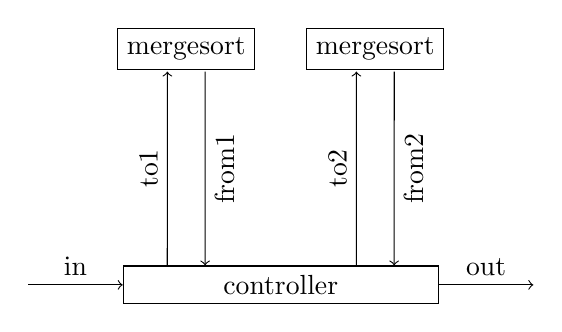
\begin{tikzpicture}[xscale = 1.2]
\draw (0,0) node[draw, minimum width=40mm] (controller) {\scalashape controller};
\draw[->] (controller.west) ++ (-1,0) -- 
   node[above]{\scalashape in} (controller.west);
\draw[<-] (controller.east)++(1,0)  -- 
   node[above]{\scalashape out} (controller.east);
%
\draw (controller) ++ (-1,3) node[draw] (rec1) {\scalashape mergesort};
\draw (rec1.south)++(-0.20,0.1) node (rec1In) {};
\draw[->] (controller.north) ++ (-1.201,0.0) -- 
  node[above,sloped] {\scalashape to1} (rec1In);
% Note: the 0.001 difference between x-coords is to get the label on the right
% side.
\draw (rec1.south)++(0.2,0.1) node (rec1Out) {};
\draw[<-] (controller.north) ++ (-0.801,0) -- 
  node[below,sloped] {\scalashape from1} (rec1Out);
%
\draw (controller) ++ (1,3) node[draw] (rec2) {\scalashape mergesort};
\draw (rec2.south)++(-0.2,0.1) node (rec2In) {};
\draw[->] (controller.north) ++ (0.8,0.0) -- 
  node[above,sloped] {\scalashape to2} (rec2In);
\draw (rec2.south)++(0.2,0.1) node (rec2Out) {};
\draw[<-] (controller.north) ++ (1.2,0) -- 
  node[below,sloped] {\scalashape from2} (rec2Out);
\end{tikzpicture}
\end{center}

%%%%%

The code in Figure~\ref{fig:mergesort} implements this strategy.  (We describe
below the |merge| function that merges the streams from the recursive
threads.)  Thus, when the input stream contains at least two elements, the
|mergesort| function runs the parallel composition of the controller and the
results of two recursive calls to |mergesort|.

\begin{figure}
\begin{scala}
  /** Merge sorted streams received on £in1£ and £in2£ into a single sorted
    * stream on £out£. */
  private def merge(in1: ??[Int], in2: ??[Int], out: !![Int]) = {
    var x1 = in1?(); var x2 = in2?(); var closed1 = false; var closed2 = false
    while(!closed1 && !closed2){
      if(x1 <= x2){ out!x1; attempt{ x1 = in1?() }{ closed1 = true } }
      else{ out!x2; attempt{ x2 = in2?() }{ closed2 = true } }
    }
    if(closed2){ out!x1; repeat{ out!(in1?()) } }
    else{ assert(closed1); out!x2; repeat{ out!(in2?()) } }
    out.endOfStream()
  }

  def mergesort(in: ??[Int], out: !![Int]): ThreadGroup = thread("mergesort"){
    var x1 = -1; var x2 = -1
    attempt{ 
      x1 = in?()
      attempt{
        x2 = in?()
        val to1, to2, from1, from2 = new SyncChan[Int]
        def controller = thread("controller"){
          to1!x1; to2!x2
          repeat{ to1!(in?()); to2!(in?()) }
          to1.endOfStream(); to2.endOfStream()
          merge(from1, from2, out)
        } // End of £controller£.
        // Put system together and run it.
        run( controller || mergesort(to1, from1) || mergesort(to2, from2) )
      }{ out!x1; out.endOfStream() } // Received only £x1£.
    }{ out.endOfStream() } // Received empty stream.
  }
\end{scala}
\caption{The concurrent mergesort program.}
\label{fig:mergesort}
\end{figure}


We now consider the |merge| function.  This will repeatedly hold two values
that it received from the two recursive |mergesort|s; it will output the
smaller, and input again from the relevant recursive |mergesort|.  However,
the definition is made harder by the fact that when one of its input streams
is closed, it will still be holding a value it received on the other input
stream: it needs to output that value, and also deal with any remaining values
in the non-closed stream.  The code does this by maintaining two boolean
variables.  The variable |closed1| is true if |in1| has been detected as
closed; otherwise |x1| holds the last value read from |in1|, which has not yet
been output.  A similar property holds for |closed2|, |x2|, and~|in2|.

%%%%%  

We now consider testing.  Testing is an important part of programming; but
since concurrent programs tend to be harder than sequential ones, testing is
particularly important in this case.

A general strategy for testing a concurrent program is to generate some random
data, run the concurrent program on it, run a corresponding sequential program
on it, and check that the two give the same answer.  This can be repeated many
times.  Of course, this assumes that we have a correct sequential program for
the same problem, but that's normally not too difficult.  In fact, this
strategy is also useful for testing sequential programs, where we have a
simple implementation that we are sure is correct, but we want to test a more
sophisticated program against it.

The following code achieves this.
%
\begin{scala}
  import scala.util.Random
  val MaxSize = 100; val Max = 100
  def doTest = {
    val size = Random.nextInt(MaxSize)
    val xs = Array.fill(size)(Random.nextInt(Max)); val ys = new Array[Int](size)
    val in, out = new SyncChan[Int]
    def sender = thread("sender"){ for(x <- xs) in!x; in.endOfStream() }
    def receiver = thread("receiver"){ 
      var i = 0; repeat{ ys(i) = out?(); i += 1 } 
    }
    run(sender || mergesort(in, out) || receiver)
    assert(xs.sorted.sameElements(ys),
      "Inputs: "+xs.mkString(", ")+"\nExpected: "+xs.sorted.mkString(", ")+
      "\nReceived: "+ys.mkString(", "))
  }
\end{scala}
%
The |doTest| function performs a single test.  If uses an array |xs| of
size~|size|, where |size| is picked randomly in the range
$\interval{0}{\sm{MaxSize}}$; each element of |xs| is picked randomly in the
range $\interval{0}{\sm{Max}}$.  The |sender| thread sends the elements
of~|xs| to the |qSort| network on the |in| channel, then signals the end of
the stream.  The |receiver| thread receives the outputs from |qSort|, and
stores them in~|ys|.  The final line tests whether a sorted version of |xs|
(sorted using the |sorted| function from the Scala |Array| class) contains the
same elements as the outputs; if this doesn't hold, it prints information
about the inputs and outputs, to help with debugging.

We can then run |doTest| many times:
%
\begin{scala}
  for(i <- 0 until 1000){ doTest; if(i%10 == 0) print(".") }
\end{scala}
%
This also intermittently prints a dot on the screen; this means that if the
system deadlocks for some reason, we will spot that it has got stuck!

There are several exercises at the end of this chapter that involve building
sorting circuits.  They can be tested in the same way.

%%%%%%%%%%%%%%%%%%%%%%%%%%%%%%%%%%%%%%%%%%%%%%%%%%%%%%%%%%%%

\section{Reasoning about the ordering of actions}

We will sometimes want to reason about the order in which particular
actions---such as memory reads and writes, and sends and receives of
messages---occur.

Consider a particular execution of a program.  We will write $a \prec a'$, to
mean that $a$ necessarily happens before~$a'$.  For example, $a$ and~$a'$
might be events performed by the same thread in that order; or they might,
respectively, be a send and receive on a buffered channel.

We will write $a \preceq a'$ to mean that $a$ happens before, or
simultaneously with, $a'$.  
%
We write $\equiv$ for the equivalence relation induced by~$\prec$:
\[\mstyle
a \equiv a' \iff a \preceq a' \land a' \preceq a.
\]
This means that $a$ and~$a'$ happen at the same time.  For example, that might
actually be the same action.  However, we also treat a send and receive on a
\emph{synchronous} channel as happening at the same time.

For example, consider the following program.
\begin{scala}
  val c = new OnePlaceBuffChan[Unit]
  run(thread{ print("Hello "); c!() } || thread{ c?(); println("world") })
\end{scala}
%
The type |Unit| contains a single value, called the unit value, denoted~|()|.
Thus communications on~|c| do not pass any data, but just send a signel.
%
We can reason about the above program using happens-before notation.  We
represent actions of the program by the corresponding program syntax.  Then in
every execution:
\[
\begin{array}{cl@{\qquad}l}
& \sm{print("Hello ")} \\
\prec & \sm{c!()} & \mbox{(program order for the first thread)} \\
\prec & \sm{c?{}} & \mbox{(ordering for a buffered channel)} \\
\prec & \sm{println("world")} & \mbox{(program order for the second thread).}
\end{array}
\]
The order of printing is as we would like. 

If we use a synchronous channel, we can reverse the send and receive:
%
\begin{scala}
  val c = new SyncChan[Unit]
  run(thread{ print("Hello "); c?() } || thread{ c!(); println("world") })
\end{scala}
%
Reasoning as before:
\[
\begin{array}{cl@{\qquad}l}
& \sm{print("Hello ")} \\
\prec & \sm{c?()} & \mbox{(program order for the first thread)} \\
\equiv & \sm{c?{}} & \mbox{(ordering for a synchronous channel)} \\
\prec & \sm{println("world")} & \mbox{(program order for the second thread).}
\end{array}
\]
In this case, the communication on~|c| acts as a synchronisation between the
two threads, without passing any data.
  
Formally, $\preceq$ is a preorder, i.e.~a transitive, reflexive order such
that:
%
\begin{itemize}
\item
If $a$ and $a'$ are actions of a single thread, and $a$ precedes $a'$ in
program order, then $a \prec a'$;

\item
If $a$ is a send and $a'$ is the corresponding receive on a buffered channel,
then $a \prec a'$;

\item
If $a$ is a send and $a'$ is the corresponding receive on a synchronous
channel, then $a \equiv a'$.
\end{itemize}

Note that some pairs of actions may be unrelated by~$\preceq$.  For example,
consider two actions in different threads, with no intervening channel
communication.  In such cases, the actions can happen in either order, so, we
need to be sure that either order is acceptable---i.e.~there is no race
condition.

Using this style of reasoning can also be useful for reasoning about the
efficiency of a concurrent program.  Suppose we can find a chain of $n$
ordered actions:
\[
\mstyle
a_1 \prec a_2 \prec \ldots \prec a_n. 
\]
Then we can be sure that the time taken for the program to complete is at
least the time to perform those $n$ actions.  Conversely, suppose we can be
sure that there is no such chain of length longer than~$n$, and suppose we run
the program on hardware such that every thread can run on its own processor,
without being descheduled; then the program will run in time $O(n)$.  Thus
finding the length of the longest such chain can give us an idea of the
running time of the program (modulo the assumption about hardware).

For example, consider the mergesort program from the previous section.  We can
consider just the actions of sending and receiving messages: between each
consecutive pair of such actions, a thread does $O(1)$ amount of work.  Let's
write $A(l)$ for the number of such actions performed on an input stream of
length~$l$.  For simplicity, let's restrict to the case where $l$ is a power
of~2.  Then we have the following equations:
%
\begin{eqnarray*}
A(1) & = & 2, \\
A(l) & = & 4l+A(l/2).
\end{eqnarray*}
%
The first equation is straightforward: the one data value is inputted and
outputted.  For the second clause, note that a maximal chain is comprised of:
the controller inputting $l$ values interleaved with $l$ sends of those values
to the recursive threads; $A(l/2)$ actions by a recursive thread; then the
controller receiving $l$ values from the recursive threads interleaved with
$l$ outputs of those values.  It is then straightforward to show that $A(l)
\le 8l$ (e.g.~via a proof by induction).  Thus we can potentially sort $l$
inputs in time $O(l)$---unlike the $O(l \log l)$ time for a sequential
program!  This result needs to be treated with a pinch of salt: the
program uses nearly~$2l$ threads, and for even moderate values for~$l$, we're
unlikely to have enough processors for every thread to run without being
descheduled. 

 


%%%%%%%%%%%%%%%%%%%%%%%%%%%%%%%%%%%%%%%%%%%%%%%%%%%%%%%%%%%%

\section{IMPROVE}

%% \heading{Data-less channels}

%% It is sometimes useful to use a channel communication solely for
%% synchronisation between threads, rather than to pass any data.

%% This can be achieved in SCL using a channel that passes data of type
%% \SCALA{Unit}, the trivial type that contains a single value~\SCALA{()}.  

%% For example:
%% \begin{scala}
%% val c = new SyncChan[Unit]
%% run(thread{ print("Hello "); c!() } || thread{ c?(); println("world") })
%% \end{scala}

%% % This usage corresponds to simple events in CSP. 
%% We can reason using the happens-before relation.
%% \[
%% \sm{print("Hello")} \prec \sm{c!()} \equiv \sm{c?()} \prec \sm{println("world")}.
%% \]

%% The use of |!| and |?| could be reversed (but not with a buffered channel).

%%%%%%%%%%%%%%%%%%%%%%%%%%%%%%%%%%%%%%%%%%%%%%%%%%%%%%%%%%%%

%%%%%

\heading{Other approaches}

\begin{itemize}
\item Concurrent Scala Objects (CSO) is an API developed by Bernard Sufrin.
  SCL is heavily based on CSO.

\item Go\footnote{\url{https://golang.org/}} is a programming language created
by Google, using CSP-style channels.  It is probably the most
mainstream such language.

\item
{\sf occam} is a programming language based on CSP, and developed by INMOS in
the early 1980s.

\item Erlang uses similar ideas, in a functional setting.

\item JCSP\footnote{\url{http://www.cs.kent.ac.uk/projects/ofa/jcsp/}} is an
implementation of CSP for Java.

% \item Eclectic
% CSP\footnote{\url{http://users.comlab.ox.ac.uk/bernard.sufrin/ECSP/ecsp.pdf}}
% is an experimental language based on CSP, and a precursor of CSO.

%% \item Communicating Haskell
%% Processes\footnote{\url{http://www.cs.kent.ac.uk/projects/ofa/chp/}} is a
%% Haskell library to support CSP-style communication.

\item Rust supports concurrency in a number of styles, including message
  passing\footnote{%
    \url{https://doc.rust-lang.org/book/ch16-02-message-passing.html}}. 

% \item
% There are various experimental languages based on Python with CSP-style
% communication. 
\end{itemize}


%%%%%


\section{Summary}

Other approaches

Encapsulation

\heading{Object-oriented versus thread-oriented programming}

Objects and threads can both be thought of as forms of
\emph{modularisation}. 

In object-oriented systems, many objects can exist simultaneously, each with
its own state.  Normally, a single one is active at a time.  They communicate
by procedure calls, which pass data and control.

In thread-oriented systems, many threads can exist simultaneously, each
with its own state, and (often) all active at the same time.  They communicate
by sending and receiving messages, which pass data.

Sometimes an individual thread will use multiple objects.  Sometimes objects
encapsulate threads.


\begin{itemize}
\item Examples: Quicksort, sorting networks.

\item 
Data-less channels.

\item
The happens-before relation.

\item
Threads and objects.

\item
Other approaches.
\end{itemize}


%%%%%


%%%%%%%%%%%%%%%%%%%%%%%%%%%%%%%%%%%%%%%%%%%%%%%%%%%%%%%% %%%%%

\section{Summary}

\begin{itemize}
\item 
Message passing using channels;

\item
Synchronous channels, buffered channels, ports, sending and receiving;

\item
Closing channels; dealing with closed channels;

\item
Examples: components; pipelines; fine-grained concurrency.
\end{itemize}


%%%%%%%%%%%%%%%%%%%%%%%%%%%%%%%%%%%%%%%%%%%%%%%%%%%%%%%

\exercises

\begin{questionS}
Implement a variant of the |NatsCircuit| program from
Figure~\ref{fig:NatsCircuit} that receives an input~|max| (say from the command
line) and produces the natural numbers up to~|max| (inclusive), and then
terminates cleanly.
\end{questionS}

\begin{answerS}
We use the |takeWhile| function from Figure~\ref{fig:BoundedMults4}, and
insert a suitable component between the |prefix 0| and |tee| components.  
\begin{scala}
  def nats(max: Int, out: !![Int]): ThreadGroup = {
    val nats, nats1, succs, back = new SyncChan[Int]
    prefix(0, succs, nats) || takeWhile((x: Int) => x <= max, nats, nats1) ||
      tee(nats1, out, back) || map((x: Int) => x+1, back, succs)
  }
\end{scala}
We also adapt the |prefix|, |tee| and |map| functions so that each closes its
output channel when its |repeat| loop terminates (strictly speaking, this
isn't necessary for |prefix|).  Thus, when the |takeWhile| component receives
a value greater than |max|, the termination signal gets passed round the
circuit.
\end{answerS}

%% \begin{scala}
%% /** A fine-grained concurrent network that prints the natural numbers up to a
%%   * limit provided on the command line. */
%% object BoundedNatsCircuit{
%%   /** Repeatedly input on `in`, printing the values received. */
%%   def console[A](in: ??[A]) = thread{ repeat{ println(in?()) } }

%%   /** Copy from `in` to `out`, prefixing with `x`. */
%%   def prefix[A](x: A, in: ??[A], out: !![A]) = thread{
%%     out!x; repeat{ out!in?() }; out.endOfStream()
%%   }

%%   /** Copy values from `in` to both `out1` and `out2`. */
%%   def tee[A](in: ??[A], out1: !![A], out2: !![A]) = thread{
%%     repeat{ val x = in?(); out1!x; out2!x }
%%     out1.endOfStream(); out2.endOfStream()
%%   }

%%   /** Apply `f` to all values received on `in`, and output on `out`. */
%%   def map[A,B](f: A => B, in: ??[A], out: !![B]) = thread{
%%     repeat{ out!(f(in?())) }; out.endOfStream()
%%   }

%%   def takeWhile[A](p: A => Boolean, in: ??[A], out: !![A]) = thread{
%%     var done = false
%%     repeat(!done){ 
%%       val x = in?(); if(p(x)) out!x else done = true
%%     }
%%     out.endOfStream()
%%   }

%%   /** The network. */
%%   def nats(max: Int, out: !![Int]): ThreadGroup = {
%%     val nats, nats1, succs, back = new SyncChan[Int]
%%     prefix(0, succs, nats) || takeWhile((x: Int) => x <= max, nats, nats1) ||
%%       tee(nats1, out, back) || map((x: Int) => x+1, back, succs)
%%   }

%%   def system(max: Int) = {
%%     val c = new SyncChan[Int]; nats(max, c) || console(c)
%%   }

%%   def main(args: Array[String]) = {
%%     val max = args(0).toInt; run(system(max))
%%   }
%% }
 % bounded version of NatsCircuit

\begin{questionS}
\label{ex:merge}
Create a component with the signature
\begin{scala}
  def merge(left: ??[Int], right: ??[Int], out: !![Int])
\end{scala}
which receives ascending streams of data on its input channels (each without
repetition), and merges them into a single ascending stream (again without
repetition).
\end{questionS}

%%%%%%%%%%%%%%%%%%%%%%%%%%%%%%%%%%%%%%%%%%%%%%%%%%%%%%%

\begin{answerS}
My code is below. 
\begin{scala}
  def merge(left: ??[Int], right: ??[Int], out: !![Int]) = thread("merge"){
    // Invariant: £l£ is the last value read from £left£; £r£ is the last value read from
    // £right£.
    var l = left?(); var r = right?()
    repeat{
      if(l < r){ out!l; l = left?() }
      else if(l == r){ out!l; l = left?(); r = right?() }
      else{ out!r; r = right?() }
    }
  }
\end{scala}
If one of the input channels closes, this simply terminates.  Arguably, the
component should continue to pass data from the input channel that is still
open, although that requires maintaining some extra state, recording whether
the values in~|l| and~|r| have been output yet.  
\end{answerS}


\begin{question}
\emph{Hamming numbers} are numbers whose only prime factors are $2$, $3$,
and~$5$.  Hence the first few Hamming numbers are:
\[ \mstyle
1, 2, 3, 4, 5, 6, 8, 9, 10, 12, 15, 16.
\]
Thus each Hamming number is either~$1$, or an earlier Hamming number
multiplied by~$2$, $3$, or~$5$.

The Hamming numbers can be produced by a circuit as depicted below.
%
\begin{center}
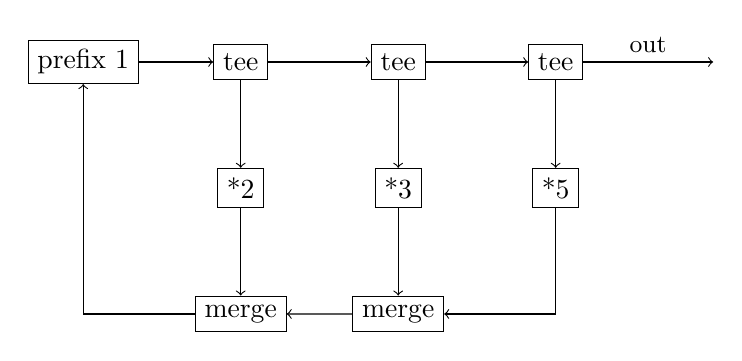
\begin{tikzpicture}[yscale = 0.8]
\draw (0,0) node[draw] (prefix) {\scalashape prefix 1};
% (*2) branch
\draw (prefix) ++ (2,0) node[draw] (tee2) {\scalashape tee};
\draw[->] (prefix) -- (tee2);
\draw (tee2) ++ (0,-2) node[draw] (mult2) {\scalashape *2};
\draw[->] (tee2) -- (mult2);
% (*3) branch
\draw (tee2) ++ (2,0) node[draw] (tee3) {\scalashape tee};
\draw[->] (tee2) -- (tee3);
\draw (tee3) ++ (0,-2) node[draw] (mult3) {\scalashape *3};
\draw[->] (tee3) -- (mult3);
% (*5) and out branch
\draw (tee3) ++ (2,0) node[draw] (tee4) {\scalashape tee};
\draw[->] (tee3) -- (tee4);
\draw (tee4) ++ (0,-2) node[draw] (mult5) {\scalashape *5};
\draw[->] (tee4) -- (mult5);
\draw[->] (tee4) -- node[above] {\small\scalashape out} ++ (2,0);
% merge of (*3) and (*5)
\draw (mult3) ++ (0,-2) node[draw] (merge1) {\scalashape merge};
\draw[->] (mult5) |- (merge1);
\draw[->] (mult3) -- (merge1);
% merge with (*2)
\draw (mult2) ++ (0,-2) node[draw] (merge2) {\scalashape merge};
\draw[->] (merge1) -- (merge2);
\draw[->] (mult2) -- (merge2);
% close loop
\draw[->] (merge2) -| (prefix);
\end{tikzpicture}
\end{center}
%
The |prefix 1| and |tee| components are as in Figure~\ref{fig:NatsCircuit}.
The |merge| components are as in Exercise~\ref{ex:merge}.  The |*2|, |*3|,
and~|*5| components multiply their inputs by~$2$, $3$ and~$5$, respectively.
Thus the |prefix 1| component sets things going; the |*2|, |*3|, and |*5|
components produce appropriate multiples; and the |merge| components merge the
streams together.

\begin{enumerate}
\item Implement the circuit using synchronous channels.  You will find that
  the system deadlocks.  Why is this?

\item Adapt the network to use buffered channels where appropriate.  Is finite
  buffering enough?

\item Adapt the network so that it produces outputs only up to some given
  maximum value, and then terminates cleanly.
\end{enumerate}
\end{question}

%%%%%%%%%%%%%%%%%%%%%%%%%%%%%%%%%%%%%%%%%%%%%%%%%%%%%%%

\begin{answerI}
I produce the system (for the final part) as follows.  The |*2|, |*3|,
and~|*5| components are simply instances of~|map|.
%
\begin{scala}
def system(out: !![Int], max: Int) = {
  val h0, h1, h2 = new SyncChan[Int]     // Inputs into £tee£ components.
  val i2, i3, i5 = new SyncChan[Int]     // Inputs into £*2£, £*3£, £*5£.
  val t2, t3, t5 = new UnboundedBuffChan[Int] // Outputs from £*2£, £*3£, £*5£.
  val m1, m2, m3 = new SyncChan[Int]    // Outputs from £merge£s and £takeWhile£.
  prefix(1, m3, h0) || tee(h0, i2, h1) || tee(h1, i3, h2) || tee(h2, i5, out) ||
  map((x:Int) => 2*x, i2, t2) || map((x:Int) => 3*x, i3, t3) || 
  map((x:Int) => 5*x, i5, t5) ||  
  merge(t2, t3, m1) || merge(t5, m1, m2) || 
  takeWhile((x: Int) => x <= max, m2, m3)
}
\end{scala}

The system without buffering deadlocks, basically because there are too many
intermediate values passing round the system for the various components to
hold.  In a bit more details, suppose the |prefix| component has just passed
a value~$n$.  Then the |*2| component will have output most of the Hamming
numbers less than $2n$; I say ``most'', because there might be a couple of
Hamming numbers either still in the |*2| component or the previous |tee|
component.  But that means that most of the Hamming numbers between $n$
and~$2n$ have to be stored somewhere in the subcircuit between the |*2| and
|prefix| components---and there simply isn't enough capacity for all of them.  
I use a buffered channel for the output from the |*2| component to store
them.  In fact, the number of Hamming numbers between~$n$ and~$2n$ tends to
infinity as $n$ tends to infinity, so we need an unbounded buffer.  The same
is true for the |*3| and |*5| components. 

To achieve termination, I inserted a |takeWhile| component just before the
|prefix| component---but it could have been inserted pretty much anywhere.  We
also adapt each component to close its output channels when its main loop
terminates, and also arrange for the |takeWhile| and |merge| components to
close their input channels; the latter is necessary, or else we can get into a
situation where one of those components is trying to send to another, but the
latter has terminated, so the network is deadlocked.  There's no harm in
\emph{every} component closing its input channels. 
\end{answerI}
 


\input{Exercises/pipesort} % sorting using a pipeline.

\begin{question}
\label{ex:sorting}
% Draw a comparator in the rows given by #1 and #2, with a horizontal
% displacement of #3
\def\comp#1#2#3{%
  \draw (#1)+(#3,0) node {$\bullet$};
  \draw (#2)+(#3,0) node (n2) {$\bullet$};
  \draw[thick] (#1)+(#3,0) -- (n2.center);
}
This question builds some networks to sort a list of numbers.  The networks
are not very sensible as software sorting networks; however, they could be
implemented efficiently in hardware. 
%%  The main aims of the practical are to help you get used to thinking about
%% concurrent systems, and to gain familiarity with the SCL library.

Each sorting network will be built from \emph{comparators}: simple
two-element sorting components.  A comparator can be pictured as below: 
%
\begin{center}
\begin{tikzpicture}[scale = 0.6, >=angle 90,shorten >=1pt]
\node at (0,0.6) {comparator};
\draw (-2,-0.5) rectangle (2,1.5);
\node (x1) at (-5, -0.2) {$x_1$};
\node (x0) at (-5, 1.2) {$x_0$};
\draw[->] (x1) -- node[above]{\scalashape\small in1} (-2,-0.2);
\draw[->] (x0) -- node[above]{\scalashape\small in0} (-2,1.2);
\node (y1) at (7.2,-0.2) {$y_1 = max(x_0,x_1)$};
\node (y0) at (7.2,1.2) {$y_0 = min(x_0,x_1)$};
\draw[->] (2,-0.2) -- node[above]{\scalashape\small out1} (y1);
\draw[->] (2,01.2) -- node[above]{\scalashape\small out0} (y0);
\end{tikzpicture}
\end{center}
%
The comparator has two input channels, |in0| and |in1|, and two output
channels, |out0| and |out1|.  If it inputs $x_0$ and~$x_1$, it outputs their
minimum on~|out0| and their maximum on~|out1|.

\begin{qpart} 
Implement a comparator with the following signature:
%
\begin{scala}
  /** A single comparator, inputting on £in0£ and £in1£, and outputting on £out0£
    * (smaller value) and £out1£ (larger value). */
  def comparator(in0: ??[Int], in1: ??[Int], out0: !![Int], out1: !![Int]): ThreadGroup
\end{scala}
%
the process should be willing to perform the inputs in either order, and
perform the outputs in either order.  The process should repeat this behaviour
until one of its channels is closed, at which point it should terminate.
\end{qpart}

%%%%%

Below is a sorting circuit for four inputs using five comparators.
%
\begin{center}
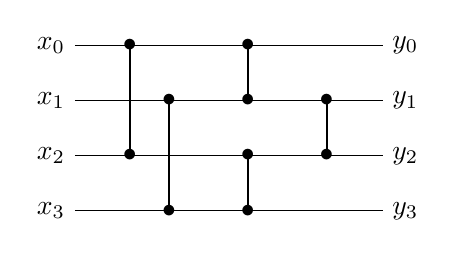
\begin{tikzpicture}[yscale = 0.7]
\draw (0,0) node (x0) {$x_0$};
\draw (0,-1) node (x1) {$x_1$};
\draw (0,-2) node (x2) {$x_2$};
\draw (0,-3) node (x3) {$x_3$};
\draw (4.5,0) node (y0) {$y_0$};
\draw (4.5,-1) node (y1) {$y_1$};
\draw (4.5,-2) node (y2) {$y_2$};
\draw (4.5,-3) node (y3) {$y_3$};
\draw (x0) -- (y0);
\draw (x1) -- (y1);
\draw (x2) -- (y2);
\draw (x3) -- (y3);
\comp{x0}{x2}{1}  \comp{x1}{x3}{1.5}
\comp{x0}{x1}{2.5}  \comp{x2}{x3}{2.5}
\comp{x1}{x2}{3.5}
\end{tikzpicture}
\end{center}
%
The first four comparators direct the smallest and largest values to the top
and bottom outputs; the final comparator sorts out the middle two values.
Note that the first two comparators can run concurrently, as can the second
pair: the longest path involves  three comparators.

\begin{qpart}
\label{Q:sort4}
Implement this sorting circuit, using the following
signature.%% \footnote{The class {\scalashape List} represents lists.  If
  %% you haven't used this class before, you might want to look at the
  %% API documentation, or a relevant on-line tutorial.}
%  
\begin{scala}
  /** A sorting network for four values. */
  def sort4(ins: List[??[Int]], outs: List[!![Int]]): ThreadGroup = {
    require(ins.length == 4 && outs.length == 4)
    ...
  }
\end{scala}
%
Test your implementation using the following idea: pick four random |Ints|,
and send them in on the input channels; receive the outputs and check that
they are a sorted version of the inputs; repeat many times.
\end{qpart}

%%%%%

We will  implement a sorting network based on the idea of insertion sort.
%
First, we need a circuit to insert a value into a sorted list of
$n \ge 1$ values, with the following signature.
%
\begin{mysamepage}
\begin{scala}
  /** Insert a value input on £in£ into a sorted sequence input on £ins£. 
    * Pre: £ins.length£ = £n£ and £outs.length = n+1£, for some £$\sm n \ge 1$£.
    * If the values £$xs$£ input on £ins£ are sorted, and £$x$£ is input on £in£, then a
    * sorted permutation of £$x::xs$£ is output on £ys£. */
  def insert(ins: List[??[Int]], in: ??[Int], outs: List[!![Int]]): ThreadGroup = {
    val n = ins.length; require(n >= 1 && outs.length == n+1)
    ...
  }
\end{scala}
\end{mysamepage}
%
Consider the circuit below to implement |insert|, for $\sm n \ge 2$.  The box
labelled ``$\sm{insert}_{\ss n-1}$'' is (recursively) a circuit to insert the
output of the comparator into the sorted list of values received on
$\sm{ins(1)}, \ldots, \sm{ins(n-1)}$. %  of length~$\sm n-1$.
%
%
\begin{center}
\def\width{6.5} % x coord for output labels
\def\recX{2} % X coord for start of recursive insert
\def\recWidth{3} % width of recursive insert
\def\recEnd{\recX+\recWidth} % X coord of right edge of recursive insert
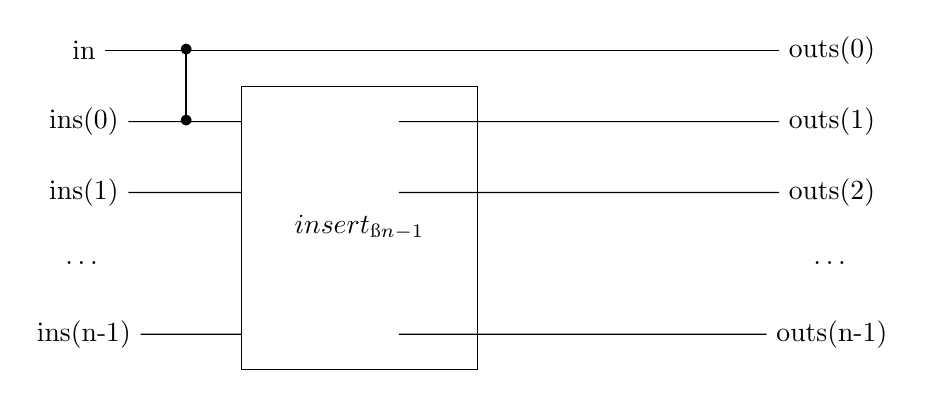
\begin{tikzpicture}[yscale = 0.9]
% First row
\draw(0,0) node (in) {\scalashape in};
\draw(\width,0) node (outs0) {\scalashape outs(0)};
\draw (in)--(outs0);
% Recursive insert box
\draw (\recX+1.5,-2.5) node {$\sm{insert}_{\ss n-1}$};
\draw (\recX,-0.5) -- ++(3,0) -- ++ (0,-4) -- ++(-3,0) -- ++ (0,4);
% Second row
\draw (0,-1) node (ins0) {\scalashape ins(0)};
\draw (ins0) -- (\recX,-1);
\comp{in}{ins0}{1.3};
\draw (\width,-1) node (outs1) {\scalashape outs(1)};
\draw (\recEnd,-1) -- (outs1);
%
\draw (0,-2) node (ins1) {\scalashape ins(1)};
\draw (ins1) -- (\recX,-2);
\draw (\width,-2) node (outs2) {\scalashape outs(2)};
\draw (\recEnd,-2) -- (outs2);
%
\draw (0,-3) node {\ldots};
\draw (\width,-3) node {\ldots};
%
\draw (0,-4) node (inslast) {\scalashape ins(n-1)};
\draw (inslast) -- (\recX,-4);
\draw (\width,-4) node (outslast) {\scalashape outs(n-1)};
\draw (\recEnd,-4) -- (outslast);
\end{tikzpicture}
\end{center}
%
\begin{qpart}
\label{Q:insert1}
Study the circuit and persuade yourself that it indeed implements the
requirements.  Then implement |insert| based upon the circuit.  You will also
need a base case, for $\sm n = 1$.  Test the circuit.
\end{qpart}

%%%%%

%% %\begin{question}
%% \label{Q:insert2}
%% \textbf{Optional:} The circuit from the previous question had a path
%% containing $O(n)$ comparators.  Design, implement and test a circuit for
%% |insert| such that the longest path has length $O(\log n)$.
%% %\end{question}

%%%%%

\begin{qpart}
Use your function from part~\ref{Q:insert1} to implement insertion sort.  Use
the following signature.
%
\begin{scala}
  /** Insertion sort. */
  def insertionSort(ins: List[??[Int]], outs: List[!![Int]]): ThreadGroup = {
    val n = ins.length; require(n >= 2 && outs.length == n)
    ...
  }
\end{scala}
%
You should base your implementation on the following cicuit, where the
sub-circuit $\sm{iSort}_{\ss n-1}$ recursively sorts $\sm n-1$ inputs.

\begin{center}
\def\width{9.5} % x coord for output labels
\def\recStart{1.5} % X coord for start of recursive iSort
\def\recWidth{2.5} % width of recursive iSort
\def\recEnd{\recStart+\recWidth} % X coord of right edge of recursive iSort
\def\insStart{5.5}
\def\insWidth{2.5}
\def\insEnd{\insStart+\insWidth}
%
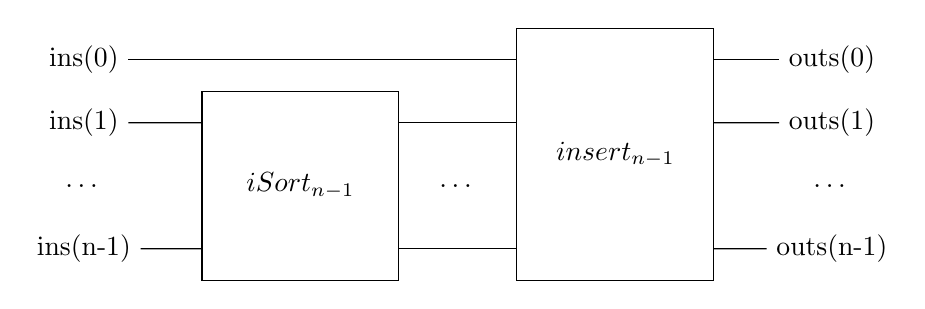
\begin{tikzpicture}[yscale = 0.8]
% Top row
\draw(0,0) node (ins0) {\scalashape ins(0)};
\draw(\width,0) node (outs0) {\scalashape outs(0)};
\draw (ins0)--(\insStart,0); \draw (\insEnd,0)--(outs0);
% Recursive iSort box
\draw (\recStart+1.25,-2.0) node {$\sm{iSort}_{\sm n-1}$};
\draw (\recStart,-0.5) -- ++(\recWidth,0) -- ++(0,-3) -- ++(-\recWidth,0) -- 
  ++(0,3);
% Insert box
\draw (\insStart+1.25,-1.5) node {$\sm{insert}_{\sm n-1}$};
\draw (\insStart,+0.5) -- ++(\insWidth,0) -- ++(0,-4) -- ++(-\insWidth,0) --
  ++(0,4);
% Second row
\draw (0,-1) node (ins1) {\scalashape ins(1)};
\draw (ins1) -- (\recStart,-1);
\draw (\recEnd,-1) -- (\insStart,-1);
\draw (\width,-1) node (outs1) {\scalashape outs(1)};
\draw (\insEnd,-1) -- (outs1);
% Third row
\draw (0,-2) node  {\ldots};
\draw (\recEnd+0.75,-2) node  {\ldots};
\draw(\width,-2) node {\ldots};
% Last row
\draw (0,-3) node (inslast) {\scalashape ins(n-1)};
\draw (inslast) -- (\recStart,-3);
\draw (\recEnd,-3) -- (\insStart,-3);
\draw (\width,-3) node (outslast) {\scalashape outs(n-1)};
\draw (\insEnd,-3) -- (outslast);
\end{tikzpicture}
\end{center}
%
Test your implementation using the ideas from part~\ref{Q:sort4}.
\end{qpart}

%%%%%

%% \subsection*{Just for fun}

%% Finally, we will implement a technique known as \emph{bitonic
%%   sorting}.  The idea is closely based on merge sort: small inputs are
%% sorted directly; larger inputs are split into two; each half is sorted
%% recursively; and the results are merged together.  For simplicity, we
%% will assume that the number of inputs is a power of~2.

%% The merging circuit can be defined recursively.  The base case is
%% straightforward.  Below is the merging circuit for eight inputs, making use of
%% two four-input merge circuits and four comparators.  It assumes that the two
%% halfs of the input, $\seq{x_0,x_1,x_2,x_3}$ and $\seq{x_4,x_5,x_6,x_7}$ are
%% each sorted, and merges them into a single sorted sequence.
%% %
%% \begin{center}
%% \begin{tikzpicture}[scale = 0.4, >=angle 90,shorten >=1pt]
%% % input wires
%% \foreach \y/\i in {4/1,3/2,2/3,1/4,-1/5,-2/6,-3/7,-4/8}
%%   \node (x\i) at (-0.6,\y){$x_{\i}$};
%% \foreach \y/\z in {4/4,3/-1,2/3,1/-2,-1/-3,-2/2,-3/-4,-4/1}
%%   \draw(0,\y) -- (4,\z);
%% % mergers
%% \draw(4,-0.5) rectangle (9,-4.5);
%% \node at (6.5,-2.5) {$Merge(4)$};
%% \draw(4,0.5) rectangle (9,4.5);
%% \node at (6.5,2.5) {$Merge(4)$};
%% % connecting wires
%% \foreach \y/\z in {4/4, 3/2, 2/-1, 1/-3, -1/3, -2/1, -3/-2, -4/-4}
%%   \draw(9,\y) -- (13,\z);
%% % comparators
%% \foreach \y/\z in {4/3, -1/-2, 2/1, -3/-4}{
%%   \draw (13,\y) node {$\bullet$};
%%   \draw (13,\z) node {$\bullet$};
%%   \draw[thick] (13,\y) -- (13,\z);
%% }
%% %\foreach \y in {3.5,1.5,-1.5,-3.5}
%%   % \draw(13,\y-0.8) rectangle (14,\y+0.8);
%% %outputs
%% \foreach \y in {4,3,2,1,-1,-2,-3,-4}
%%   \draw(13,\y) -- (15,\y);
%% \foreach \y/\i in {4/1,3/2,2/3,1/4,-1/5,-2/6,-3/7,-4/8}
%%   \node at (15.5,\y){$y_{\i}$};
%% \end{tikzpicture}
%% \end{center}
%% %
%% Each half of the input is split between the two sub-merges.  Corresponding
%% outputs from the two sub-merges are fed into comparators.

%% %\begin{question}
%% Implement this sorting algorithm.  Use the following signature, for a circuit
%% for $2^k$ values.
%% %
%% \begin{scala}
%%   /** A merging network for £$2^k$£ values.  If the values received on
%%     * ins1 and ins2 are sorted, then their merger is output on outs. */
%%   def merge(k: Int)(ins1: List[?[Int]], ins2: List[?[Int]], outs: List[![Int]])
%%       : ThreadGroup = {
%%     val n = 1 << k; val halfN = n/2
%%     require(k >= 1 && ins1.length == halfN && ins2.length == halfN &&
%%               outs.length == n)
%%     ...
%%   }
%% \end{scala}
%% %
%% You might want to use the following function for doing the splitting.
%% \begin{scala}
%%   /** Split xs into two lists, alternately.
%%     * @return the lists <xs(0), xs(2), xs(4),...> and <xs(1), xs(3), xs(5), ...>
%%     */
%%   private def split[T](xs: List[T]): (List[T], List[T]) = 
%%     if(xs.isEmpty) (List[T](), List[T]())
%%     else{ val (ys, zs) = split(xs.tail); (xs.head::zs, ys) }
%% \end{scala}
%% %\end{question}

%% %%%%%

%% The sorting circuit itself can also be defined recursively.  The base case is
%% straightforward.  The recursive case is illustrated below: the input is split
%% in half; each half is sorted; the results are merged.
%% % 
%% \begin{center}
%% \begin{tikzpicture}[scale = 0.4, >=angle 90,shorten >=1pt]
%% \foreach \y in {4,3,2,1,-1,-2,-3,-4}
%%   \draw(0,\y) -- (1,\y);
%% \draw(1,0.5) rectangle (6,4.5);
%% \node at (3.5,2.5) {$sort(n)$};
%% \draw(1,-0.5) rectangle (6,-4.5);
%% \node at (3.5,-2.5) {$sort(n)$};
%% \foreach \y in {4,3,2,1,-1,-2,-3,-4}
%%   \draw(6,\y) -- (8,\y);
%% \draw(8,-4.5) rectangle (14,4.5);
%% \node at (11,0){$merge(2n)$};
%% \foreach \y in {4,3,2,1,0,-1,-2,-3,}
%%   \draw(14,\y-0.5) -- (15,\y-0.5);
%% \end{tikzpicture}
%% \end{center}

%% %\begin{question}
%% Implement this sorting circuit.  Use the following signature.
%% %% \footnote{You
%%   %% might want to use the operations {\scalashape take} and {\scalashape drop}
%%   %% from the {\scalashape List} class for splitting the input.}
%% %
%% \begin{scala}
%%   /** A bitonic sorting network for 2^k values. */
%%   def bitonicSort(k: Int)(ins: List[?[Int]], outs: List[![Int]]): ThreadGroup = {
%%     val n = 1 << k
%%     require(ins.length == n && outs.length == n)
%%     ...
%%   }
%% \end{scala}

%% Test your implementation using the ideas from Question~\ref{Q:sort4}.
%\end{question}
\end{question}

%%%%%%%%%%%%%%%%%%%%%%%%%%%%%%%%%%%%%%%%%%%%%%%%%%%%%%%

\begin{answerI}
Most of the code consists of fairly straightforward translations of the
diagrams. 
%
\begin{enumerate}
\item
%\begin{qpart}
\begin{scala}
  def comparator(in0: ??[Int], in1: ??[Int], out0: !![Int], out1: !![Int])
    = thread("comparator"){
    var x0 = -1; var x1 = -1
    repeat{
      run(thread{ x0 = in0?() } || thread{ x1 = in1?() })
      run(thread{ out0!(x0 min x1) } || thread{ out1!(x0 max x1) })
    }
    in0.close(); in1.close(); out0.endOfStream(); out1.endOfStream()
  }
\end{scala}
%\end{qpart}

%%%%%

\item
%\begin{qpart}
\begin{scala}
  def sort4(ins: List[??[Int]], outs: List[!![Int]]): ThreadGroup = {
    require(ins.length == 4 && outs.length == 4)
    val c0, c1, c2, c3, c4, c5 = new SyncChan[Int]
    comparator(ins(0), ins(2), c0, c2) ||
      comparator(ins(1), ins(3), c1, c3) ||
      comparator(c0, c1, outs(0), c4) ||
      comparator(c2, c3, c5, outs(3)) ||
      comparator(c4, c5, outs(1), outs(2))
  }
\end{scala}
%\end{qpart}

\item
\begin{scala}
  def insert(ins: List[??[Int]], in: ??[Int], outs: List[!![Int]])
      : ThreadGroup = {
    val n = ins.length; require(n >= 1 && outs.length == n+1)
    if(n == 1) comparator(ins(0), in, outs(0), outs(1))
    else{
      val c = new SyncChan[Int]
      comparator(in, ins(0), outs(0), c) || insert(ins.tail, c, outs.tail)
    }
  }
\end{scala}


\item
\begin{scala}
  def insertionSort(ins: List[??[Int]], outs: List[!![Int]]): ThreadGroup = {
    val n = ins.length; require(n >= 2 && outs.length == n)
    if(n == 2) comparator(ins(0), ins(1), outs(0), outs(1))
    else{
      val mids = List.fill(n-1)(new SyncChan[Int])
      insertionSort(ins.tail, mids) || insert(mids, ins(0), outs))
    }
  }
\end{scala}
\end{enumerate}
\end{answerI}
 % sorting using comparators


More exercises:

quicksort

fibs

integrator?

Bitonic part of sorting practical.

%% Nats circuit from B's notes?? 
%% \url{https://www.cs.ox.ac.uk/teaching/materials15-16/concurrentprogramming/Lectures/04-channels.pdf}
